\section{Results and discussion}
\label{sec:results}

We evaluate GLPE and GLPE (no gate), alongside intrinsic-reward baselines, on the five-environment suite from Section~\ref{sec:experimental_setup}.
Across the suite, GLPE (no gate) is a strong default: it matches the strongest baseline within uncertainty on \textsc{Humanoid-v5} and remains within a modest margin of the best baseline on \textsc{HalfCheetah-v5} and \textsc{BipedalWalker-v3} (Table~\ref{tab:final_returns_glpe_vs_baselines}).
The full gated variant is most valuable in sparse reward, where it provides a targeted guardrail against unproductive shaping; this is clearest on \textsc{MountainCar-v0}, where it achieves the best final return and reaches the solved threshold in all seeds (Tables~\ref{tab:final_returns_glpe_vs_baselines} and~\ref{tab:solved_threshold_stats}).
All plots and aggregates use the deterministic evaluation protocol: at each checkpoint we run 20 episodes per seed and report the mean \emph{extrinsic} return (i.e., the task reward without intrinsic shaping).
Unless otherwise noted, each environment uses 8 random seeds (10 for \textsc{MountainCar-v0} and 5 for \textsc{Humanoid-v5}).
We primarily interpret learning curves (Figure~\ref{fig:eval_curves_baselines}), sample efficiency via step-AUC over environment steps (Table~\ref{tab:auc_steps_glpe_vs_baselines}), thresholded reliability and steps-to-threshold (Figure~\ref{fig:steps_to_threshold_baselines} and Tables~\ref{tab:half_solved_threshold_stats} and~\ref{tab:solved_threshold_stats}), and wall-clock efficiency via time-AUC under a common budget (Figure~\ref{fig:eval_auc_time}).
We additionally use the training-time decomposition of extrinsic versus intrinsic rollout reward (Figure~\ref{fig:train_reward_decomp_baselines}) to contextualize how strongly intrinsic shaping influences the optimization signal.
GLPE-specific diagnostics visualize the intrinsic taper schedule (Figure~\ref{fig:glpe_intrinsic_taper}) and where gating suppresses shaping along final-checkpoint trajectories (Figure~\ref{fig:glpe_gate_map}).
Table~\ref{tab:final_returns_glpe_vs_baselines} reports final-checkpoint returns, and Table~\ref{tab:glpe_component_ablation_returns} summarizes intrinsic-component ablations on three representative tasks.

Some diagnostic and efficiency plots additionally include auxiliary GLPE variants (a cached-gate implementation and single-component ablations) to interpret compute and signal contributions; we treat these as supporting analyses rather than primary baselines.

\begin{figure*}[t]
\centering

\includegraphics[width=\linewidth,height=0.72\textheight,keepaspectratio]{figures/eval-curves-baselines-curves.png}
\caption{
Evaluation learning curves for GLPE and baseline intrinsic-reward methods.
Each panel plots mean \emph{extrinsic} return (higher is better) versus environment steps for one task.
Solid lines show the mean across seeds at each checkpoint; markers show the corresponding per-seed means (20 evaluation episodes per checkpoint).
The horizontal dashed line is a fixed ``solved'' return threshold used for summary analyses.
These curves summarize both learning speed and cross-seed stability; in particular, tight clustering of per-seed markers indicates robust performance.
}
\label{fig:eval_curves_baselines}
\end{figure*}

\begin{table}[t]
\centering
\small
\begin{tabular}{lccc}
\hline
Environment & GLPE & GLPE (no gate) & Best baseline \\
\hline
\textsc{MountainCar-v0} & $-96.2\;[-96.5,-95.9]$ & $-97.1\;[-99.0,-96.0]$ & RIAC: $-106.6\;[-127.5,-95.9]$ \\
\textsc{BipedalWalker-v3} & $266.5\;[214.0,301.3]$ & $294.4\;[285.9,303.7]$ & Vanilla PPO: $302.2\;[291.2,309.4]$ \\
\textsc{Ant-v5} & $4{,}961\;[4{,}421,5{,}359]$ & $4{,}961\;[4{,}436,5{,}349]$ & RIAC: $5{,}384\;[5{,}118,5{,}625]$ \\
\textsc{HalfCheetah-v5} & $6{,}889\;[6{,}565,7{,}285]$ & $6{,}908\;[6{,}548,7{,}280]$ & RIDE: $7{,}106\;[6{,}901,7{,}299]$ \\
\textsc{Humanoid-v5} & $1{,}970\;[546,4{,}355]$ & $2{,}858\;[1{,}428,4{,}454]$ & ICM: $2{,}874\;[770,4{,}956]$ \\
\hline
\end{tabular}
\caption{
Mean extrinsic return at the final checkpoint (latest by environment steps).
Values are means over seeds; each seed is evaluated for 20 deterministic (mode) episodes, and confidence intervals are 95\% bootstrap intervals over seeds.
Higher is better; for \textsc{MountainCar-v0} this corresponds to less negative return.
The best baseline is selected (per environment) among Vanilla PPO, ICM, RND, RIDE, and RIAC by highest mean return.
}
\label{tab:final_returns_glpe_vs_baselines}
\end{table}

\begin{table}[!hbp]
\centering
\small
\begin{fitwidthtabular}{lccc}
\hline
Environment & GLPE & GLPE (no gate) & Best baseline \\
\hline
\textsc{MountainCar-v0} & $-107.0\;[-114.8,-101.8]$ & $-111.3\;[-128.7,-101.4]$ & RIDE: $-113.7\;[-134.2,-101.9]$ \\
\textsc{BipedalWalker-v3} & $249.0\;[223.9,270.7]$ & $255.2\;[230.0,275.6]$ & ICM: $257.3\;[229.4,278.3]$ \\
\textsc{Ant-v5} & $3{,}402\;[3{,}067,3{,}708]$ & $3{,}402\;[3{,}067,3{,}707]$ & RND: $3{,}565\;[3{,}202,3{,}876]$ \\
\textsc{HalfCheetah-v5} & $5{,}005\;[4{,}708,5{,}316]$ & $4{,}998\;[4{,}700,5{,}296]$ & RIDE: $5{,}208\;[5{,}019,5{,}410]$ \\
\textsc{Humanoid-v5} & $1{,}583\;[551,3{,}360]$ & $1{,}665\;[769,2{,}921]$ & ICM: $1{,}781\;[829,2{,}797]$ \\
\hline
\end{fitwidthtabular}
\caption{
Step-AUC of deterministic evaluation return versus cumulative environment steps, computed by trapezoidal integration of the mean return--by--steps curve over evaluation checkpoints and dividing by the environment's step budget.
This yields the average evaluation return over training, rewarding methods that learn quickly and sustain high returns.
Intervals are obtained by integrating the per-checkpoint 95\% bootstrap confidence bands over seeds and should be interpreted as an approximate uncertainty range for the integrated metric.
Higher is better.
The best baseline is selected (per environment) among Vanilla PPO, ICM, RND, RIDE, and RIAC by highest mean step-AUC.
}
\label{tab:auc_steps_glpe_vs_baselines}
\end{table}


Table~\ref{tab:auc_steps_glpe_vs_baselines} summarizes interaction efficiency using a normalized step-AUC over environment steps, rewarding methods that learn quickly and sustain high returns over the fixed step budget.
By this metric, GLPE has the strongest point estimate on \textsc{MountainCar-v0}, and GLPE (no gate) remains near the top on \textsc{BipedalWalker-v3}.
On \textsc{Ant-v5} and \textsc{HalfCheetah-v5}, the GLPE variants fall within a small gap of the strongest baseline step-AUC, while \textsc{Humanoid-v5} shows a larger gap that is hard to interpret cleanly given the high across-seed variance.
We therefore treat GLPE (no gate) as the low-friction default that removes gating-specific thresholding, and view the gated variant as an optional guardrail when intrinsic shaping risks being unproductive or destabilizing in sparse-reward settings.
On \textsc{MountainCar-v0}, GLPE achieves the best final return and the strongest step-AUC (Tables~\ref{tab:final_returns_glpe_vs_baselines} and~\ref{tab:auc_steps_glpe_vs_baselines}), and both GLPE variants reach the solved threshold in all seeds (Table~\ref{tab:solved_threshold_stats}).
Several baselines exhibit occasional failures that remain near the minimum return (Figure~\ref{fig:eval_curves_baselines}), so even the most reliable baseline falls short of perfect success (Table~\ref{tab:solved_threshold_stats}).

On the MuJoCo locomotion tasks, GLPE (no gate) remains competitive with the strongest intrinsic baselines.
On \textsc{HalfCheetah-v5}, both GLPE variants track the strongest intrinsic baselines throughout training (Figure~\ref{fig:eval_curves_baselines}) and finish close to the best-performing baseline at the final checkpoint (Table~\ref{tab:final_returns_glpe_vs_baselines}).
RIDE attains the highest mean final return, but GLPE (no gate) remains close and exhibits a consistent ordering under step-AUC (Tables~\ref{tab:final_returns_glpe_vs_baselines} and~\ref{tab:auc_steps_glpe_vs_baselines}).
On \textsc{Humanoid-v5}, variance is substantial across all methods: a small number of seeds achieve high returns while others remain far below the solved threshold, leading to wide confidence intervals (Figure~\ref{fig:eval_curves_baselines}).
In this regime, GLPE (no gate) has a similar point estimate to the strongest baseline (ICM) at the final checkpoint with broadly overlapping bootstrap intervals (Table~\ref{tab:final_returns_glpe_vs_baselines}); the threshold analysis below shows that many runs reach competent behavior without consistently clearing the full solved cutoff.
The gated variant improves over vanilla PPO on average but lags GLPE (no gate), suggesting that conservative gating can be counterproductive when progress is already dominated by seed-to-seed variability.

\textsc{Ant-v5} highlights a complementary regime where dense extrinsic reward already provides strong guidance and many methods approach the solved threshold.
GLPE and GLPE (no gate) match each other closely and reach the solved threshold in most seeds, but finish modestly below the strongest baseline at the final checkpoint (Tables~\ref{tab:final_returns_glpe_vs_baselines} and~\ref{tab:solved_threshold_stats}).
The step-AUC summary mirrors this pattern, suggesting that the gap reflects lower average performance rather than being confined to the final checkpoint (Table~\ref{tab:auc_steps_glpe_vs_baselines}).
Finally, on \textsc{BipedalWalker-v3} (solved threshold $300$), GLPE (no gate) approaches the cutoff with a comparatively tight confidence interval, but many runs plateau just below $300$ (Table~\ref{tab:final_returns_glpe_vs_baselines}).
As a result, binary ``solved'' counts are highly sensitive to small between-seed differences (Tables~\ref{tab:half_solved_threshold_stats} and~\ref{tab:solved_threshold_stats}).
The gated variant increases solved-threshold reach relative to GLPE (no gate) but exhibits occasional low-return failures (Figure~\ref{fig:eval_curves_baselines}), which pull down its mean.
Taken together, \textsc{BipedalWalker-v3} illustrates a near-threshold regime where GLPE (no gate) is stable and efficient but not consistently ``pushed'' over a sharp solved cutoff.

To connect these per-environment regimes to GLPE's design choices, we use diagnostic ablations within the GLPE family---run on \textsc{MountainCar-v0}, \textsc{BipedalWalker-v3}, and \textsc{Ant-v5}---to isolate which intrinsic components matter in sparse-reward, near-threshold, and dense-reward settings.
Table~\ref{tab:glpe_component_ablation_returns} isolates the two intrinsic components by setting impact-only ($\alpha_{\mathrm{LP}}{=}0$) or LP-only ($\alpha_{\mathrm{impact}}{=}0$).
On \textsc{MountainCar-v0}, both single-term variants fall well short of GLPE, consistent with impact and learning progress acting as complementary drivers of exploration in a sparse-reward setting.
In contrast, on \textsc{Ant-v5} the impact-only variant slightly exceeds GLPE in mean final return, and on \textsc{BipedalWalker-v3} the LP-only variant comes closest to the solved threshold.
Together, these ablations suggest that while a single component can be sufficient in some dense-reward regimes, the combined GLPE score provides a robust default that avoids committing to an environment-specific choice of intrinsic signal.

\begin{table}[t]
\centering
\small
\begin{tabular}{lccc}
\hline
Environment & GLPE & Impact-only & LP-only \\
\hline
\textsc{MountainCar-v0}    & $-96.2\;[-96.5,-95.9]$        & $-111.8\;[-137.0,-96.2]$      & $-106.6\;[-127.4,-96.0]$ \\
\textsc{BipedalWalker-v3}  & $266.5\;[214.0,301.3]$       & $277.5\;[256.0,296.5]$       & $298.8\;[285.5,308.1]$ \\
\textsc{Ant-v5}            & $4{,}961\;[4{,}421,5{,}359]$  & $5{,}233\;[4{,}544,5{,}663]$  & $4{,}599\;[3{,}617,5{,}401]$ \\
\hline
\end{tabular}
\caption{
Final-checkpoint mean extrinsic return for GLPE and component ablations.
Impact-only sets $\alpha_{\mathrm{LP}}{=}0$ and LP-only sets $\alpha_{\mathrm{impact}}{=}0$.
Brackets show 95\% bootstrap confidence intervals over training seeds.
Higher is better (less negative is better on \textsc{MountainCar-v0}).
}
\label{tab:glpe_component_ablation_returns}
\end{table}


To make the gating behavior concrete, Figure~\ref{fig:glpe_gate_map} shows where the GLPE gate suppresses intrinsic shaping along trajectories from the final checkpoint.
Across environments, the gate switches off only in localized regions of the visited state distribution, supporting the interpretation of gating as a targeted backstop: it can prevent unhelpful shaping in sparse-reward settings without broadly suppressing exploration when dense reward already provides strong guidance.

\begin{figure*}[h]
\centering

\includegraphics[width=\linewidth,height=0.72\textheight,keepaspectratio]{figures/glpe-gate-map.png}
\caption{
State-space view of GLPE's gating decisions.
Points are states visited in trajectories from the final checkpoint (subsampled); for \textsc{MountainCar-v0} we plot raw position and velocity, and for the remaining environments we project z-scored observations onto the first two principal components.
Blue points indicate timesteps where the intrinsic term is active (gate on), while orange points indicate where the gate disables intrinsic shaping (gate off).
Across tasks, gate-off points occupy a small and typically localized subset of the visited distribution, indicating that gating suppresses intrinsic shaping only in narrow regions rather than globally.
}
\label{fig:glpe_gate_map}
\end{figure*}


\begin{figure*}[t]
\centering

\includegraphics[width=\linewidth,height=0.72\textheight,keepaspectratio]{figures/steps-to-beat-baselines.png}
\caption{
Sample efficiency and reliability at fixed return thresholds.
For each task, bars report the median number of environment steps required to first reach a target return level, computed by linearly interpolating between evaluation checkpoints.
The three x-axis positions correspond to 25\%, 50\%, and 100\% of that task's solved threshold (the dashed line in Figure~\ref{fig:eval_curves_baselines}); for tasks with negative solved thresholds (MountainCar), the intermediate thresholds are defined by the same monotonic mapping used in the plotting code.
Error bars show the standard deviation of steps among seeds that reached the threshold.
Bar opacity encodes the fraction of seeds that reached the threshold by the end of training, and the number above each bar is the count of successful seeds.
Lower bars and higher opacities indicate faster and more reliable learning.
}
\label{fig:steps_to_threshold_baselines}
\end{figure*}

\begin{table}[t]
\centering
\small
\begin{tabular}{lccc}
\hline
Environment & GLPE & GLPE (no gate) & Most reliable baseline \\
\hline
\textsc{MountainCar-v0} & \(10/10;\;0.12\,\mathrm{M}\) & \(10/10;\;0.11\,\mathrm{M}\) & RIDE: \(9/10;\;0.13\,\mathrm{M}\) \\
\textsc{BipedalWalker-v3} & \(8/8;\;0.44\,\mathrm{M}\) & \(8/8;\;0.41\,\mathrm{M}\) & ICM: \(8/8;\;0.41\,\mathrm{M}\) \\
\textsc{Ant-v5} & \(8/8;\;4.61\,\mathrm{M}\) & \(8/8;\;4.61\,\mathrm{M}\) & RND: \(8/8;\;4.18\,\mathrm{M}\) \\
\textsc{HalfCheetah-v5} & \(8/8;\;2.01\,\mathrm{M}\) & \(8/8;\;2.01\,\mathrm{M}\) & Vanilla: \(8/8;\;1.28\,\mathrm{M}\) \\
\textsc{Humanoid-v5} & \(2/5;\;14.51\,\mathrm{M}\) & \(4/5;\;11.47\,\mathrm{M}\) & ICM: \(4/5;\;10.32\,\mathrm{M}\) \\
\hline
\end{tabular}
\caption{
Intermediate-threshold reliability and speed.
Each cell reports the number of seeds that reached 50\% of the task's solved-return threshold by the end of training and the median training steps (in millions) to first reach that level, computed by linearly interpolating between deterministic evaluation checkpoints (Figure~\ref{fig:steps_to_threshold_baselines}).
For tasks with negative solved thresholds (MountainCar), the 50\% level uses the same monotonic mapping as in Figure~\ref{fig:steps_to_threshold_baselines}.
Medians are taken over successful seeds only.
The ``most reliable baseline'' is selected among Vanilla PPO, ICM, RND, RIDE, and RIAC by highest reach count (ties broken by lower median steps).
Higher reach counts and lower median steps indicate more reliable and faster progress toward competent performance.
}
\label{tab:half_solved_threshold_stats}
\end{table}

\begin{table}[t]
\centering
\small
\begin{tabular}{lccc}
\hline
Environment & GLPE & GLPE (no gate) & Most reliable baseline \\
\hline
\textsc{MountainCar-v0} & \(10/10;\;0.35\,\mathrm{M}\) & \(10/10;\;0.35\,\mathrm{M}\) & RIDE: \(9/10;\;0.44\,\mathrm{M}\) \\
\textsc{BipedalWalker-v3} & \(4/8;\;3.10\,\mathrm{M}\) & \(2/8;\;3.04\,\mathrm{M}\) & RIAC: \(8/8;\;4.09\,\mathrm{M}\) \\
\textsc{Ant-v5} & \(7/8;\;10.39\,\mathrm{M}\) & \(7/8;\;10.39\,\mathrm{M}\) & RIAC: \(8/8;\;10.22\,\mathrm{M}\) \\
\textsc{HalfCheetah-v5} & \(8/8;\;9.68\,\mathrm{M}\) & \(8/8;\;9.42\,\mathrm{M}\) & RIDE: \(8/8;\;9.03\,\mathrm{M}\) \\
\textsc{Humanoid-v5} & \(1/5;\;6.73\,\mathrm{M}\) & \(2/5;\;18.23\,\mathrm{M}\) & ICM: \(2/5;\;13.93\,\mathrm{M}\) \\
\hline
\end{tabular}
\caption{
Reliability and speed at the solved threshold.
Each cell reports the number of seeds that reached the task's solved threshold by the end of training and the median steps (in millions) to first reach it, computed by linearly interpolating between deterministic evaluation checkpoints (Figure~\ref{fig:steps_to_threshold_baselines}).
Medians are taken over successful seeds only.
The ``most reliable baseline'' is the method with the highest solve count among Vanilla PPO, ICM, RND, RIDE, and RIAC (ties broken by lower median steps).
}
\label{tab:solved_threshold_stats}
\end{table}


The threshold-based analysis in Figure~\ref{fig:steps_to_threshold_baselines} complements the learning curves by separating \emph{how fast} a method reaches a target score from \emph{how often} it reaches it.
We use fixed solved-return thresholds for these summaries (\textsc{MountainCar-v0}: $-110$, \textsc{BipedalWalker-v3}: $300$, \textsc{Ant-v5}: $5{,}000$, \textsc{HalfCheetah-v5}: $6{,}000$, \textsc{Humanoid-v5}: $3{,}000$), shown as dashed lines in Figure~\ref{fig:eval_curves_baselines}.
To provide a less brittle anchor than the binary ``solved'' cutoff, Table~\ref{tab:half_solved_threshold_stats} summarizes success counts and median steps at 50\% of each task's solved threshold (the middle x-axis position in Figure~\ref{fig:steps_to_threshold_baselines}), while Table~\ref{tab:solved_threshold_stats} reports the full solved threshold (the 100\% level).
At the 50\% level, GLPE (no gate) reaches the target in all seeds on four environments and in 4/5 seeds on \textsc{Humanoid-v5}, matching the best baseline reach count on every task; the gated variant is similarly reliable except on \textsc{Humanoid-v5} (2/5).
Comparing the 50\% and 100\% summaries shows that the main remaining failures are concentrated in final-threshold crossing on high-variance tasks: on \textsc{BipedalWalker-v3} and \textsc{Humanoid-v5}, many runs reach competent behavior but fewer cross the full solved cutoff (Table~\ref{tab:solved_threshold_stats}).
This pattern is consistent with GLPE's design as a transient exploration aid: it reliably supports progress toward competent behavior, but does not guarantee the last increment of performance needed to clear a hard ``solved'' cutoff without additional tuning.

Because the GLPE family anneals intrinsic shaping with a cosine taper (Section~\ref{sec:method}), its intrinsic contribution is intentionally transient.
Figure~\ref{fig:glpe_intrinsic_taper} shows that the underlying intrinsic signal remains nonzero, but the taper weight drives the applied intrinsic reward smoothly toward (near) zero as training approaches the final phase.
This behavior is visible in the optimization signal: Figure~\ref{fig:train_reward_decomp_baselines} decomposes the mean rollout reward during training into extrinsic and intrinsic components, showing that GLPE and GLPE (no gate) reduce the intrinsic term late in training while several baselines maintain a nonzero intrinsic component throughout.

\begin{figure}[t]
    \centering
    
\includegraphics[width=\linewidth]{figures/glpe-intrinsic-taper.png}
    \caption{Intrinsic annealing in the GLPE family via the cosine taper from Section~\ref{sec:method}. The dashed curve (right axis) is the taper weight applied over training progress; the solid curve (left axis) is the batch-mean intrinsic reward actually added to PPO after scaling and clipping. The dotted curve rescales this intrinsic term to factor out the taper weight, illustrating that annealing---not a collapse of the intrinsic signal---drives the intrinsic contribution toward zero as training approaches the final phase.}
    \label{fig:glpe_intrinsic_taper}
\end{figure}


\begin{figure*}[tp]
\centering
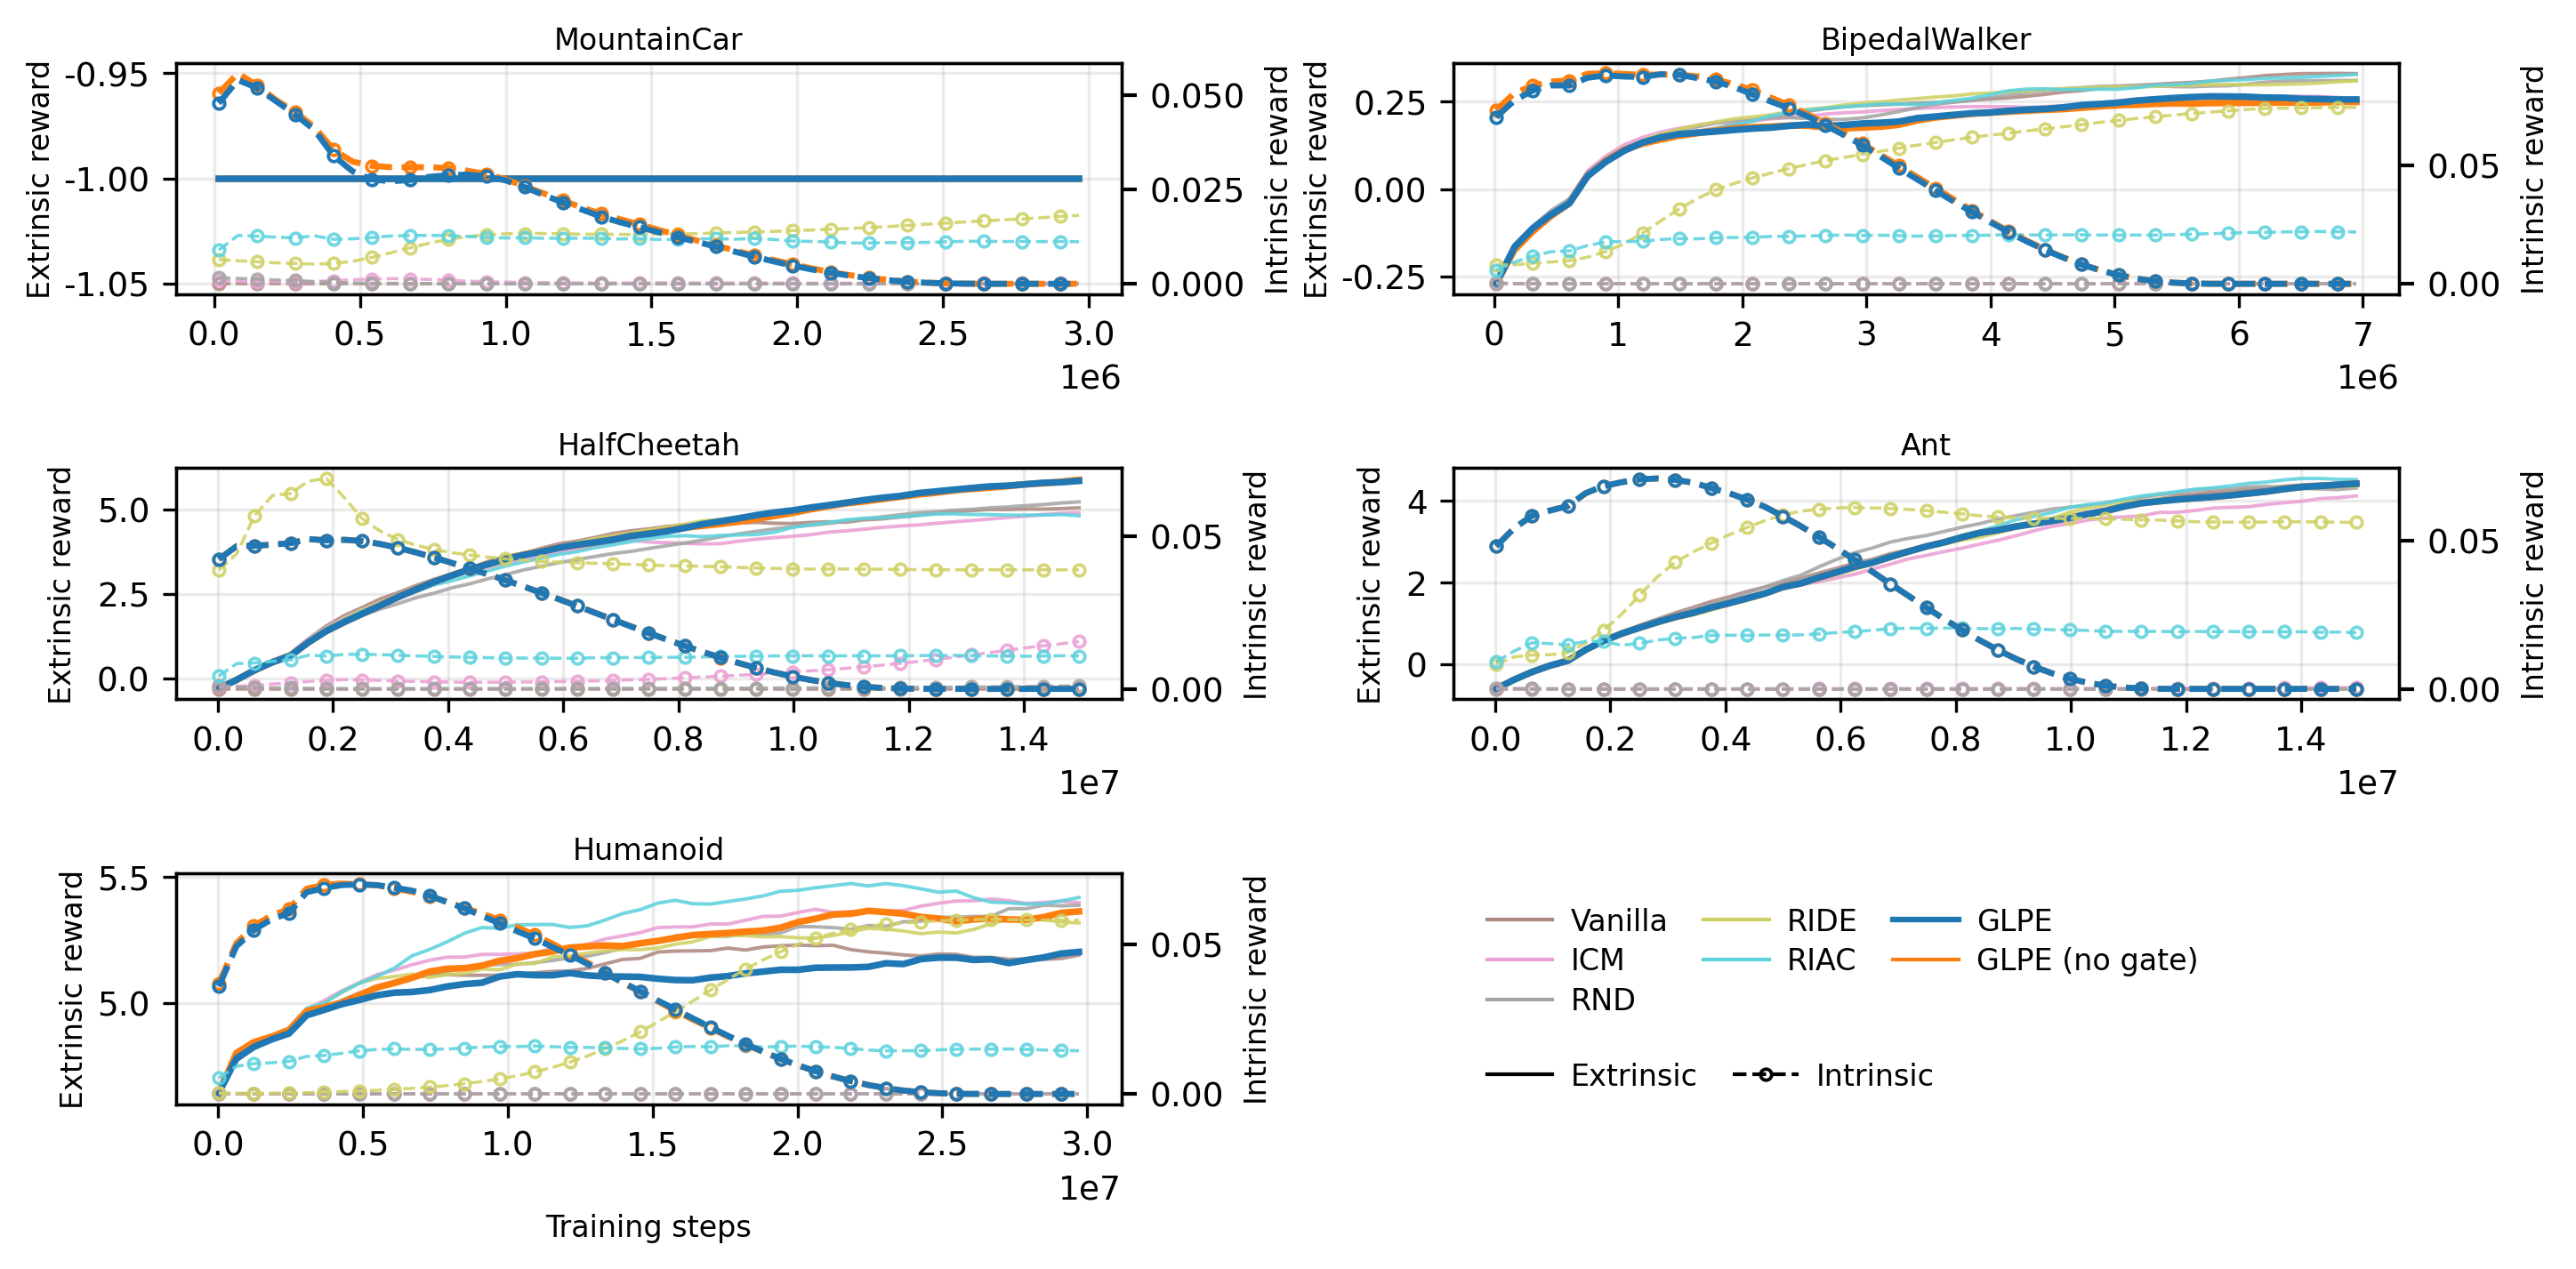
\includegraphics[width=\glpefigwidth,height=\glpefigheight,keepaspectratio]{figures/train-reward-decomp-baselines.png}
\caption{
Training-time decomposition of rollout reward.
Solid lines show the mean extrinsic reward per environment step collected during PPO rollouts.
Dashed lines show the intrinsic shaping component actually added during training, computed as the difference between the logged total reward and the extrinsic reward (after each method's scaling and clipping; GLPE additionally applies tapering).
Intrinsic values use the right axis and extrinsic values use the left axis.
This plot is a diagnostic for the optimization signal and is complementary to the evaluation curves, which report extrinsic return without intrinsic shaping.
}
\label{fig:train_reward_decomp_baselines}
\end{figure*}


\begin{figure*}[t]
\centering

\includegraphics[width=\linewidth]{figures/eval-auc-time-all-methods.png}
\caption{
Wall-clock AUC of evaluation performance.
For each task, bars report trapezoidal area-under-curve (AUC) of the mean deterministic evaluation return as a function of cumulative training time (Section~\ref{sec:experimental_setup:efficiency}).
To compare methods fairly when overhead differs, each task uses a common time horizon equal to the minimum final training time among the compared methods, and curves are truncated to this horizon (no extrapolation).
Higher is better; for tasks with negative returns (MountainCar), less-negative values yield higher (less-negative) AUC.
Error bars are derived by integrating the per-checkpoint 95\% confidence bounds on mean return.
}
\label{fig:eval_auc_time}
\end{figure*}


Computational efficiency can alter conclusions when methods are compared under a fixed wall-clock budget rather than a fixed interaction budget.
Figure~\ref{fig:eval_auc_time} summarizes this perspective using an area-under-curve (AUC) metric of evaluation return versus cumulative training time (Section~\ref{sec:experimental_setup:efficiency}), with each environment using a common time horizon to avoid extrapolating slower methods.
Across \textsc{BipedalWalker-v3}, \textsc{HalfCheetah-v5}, \textsc{Ant-v5}, and \textsc{Humanoid-v5}, GLPE (no gate) remains close to the strongest baseline in time-AUC (Figure~\ref{fig:eval_auc_time}).
Full GLPE is typically further back under this wall-clock lens, consistent with its higher per-update intrinsic overhead (Figure~\ref{fig:timing_breakdown}).
\textsc{MountainCar-v0} is more sensitive because environment stepping is comparatively cheap, so intrinsic overhead can materially affect wall-clock rankings; in this regime the time-AUC differences among the top methods are smaller than in the step-normalized view.

\begin{figure*}[t]
\centering

\includegraphics[width=\linewidth]{figures/timing-breakdown.png}
\caption{
Timing breakdown per PPO update.
Each panel shows a stacked decomposition of wall-clock seconds per training update for one task.
For each method, we take the final quarter of recorded updates in each run, compute per-component medians, and then average these medians across runs (stacked bars).
The black error bar on each stack is a 95\% confidence interval for the total seconds per update across runs.
This view helps interpret wall-clock tradeoffs: larger intrinsic segments indicate greater exploration-computation overhead, while large environment-step segments indicate simulation-dominated regimes.
}
\label{fig:timing_breakdown}
\end{figure*}

\begin{table*}[t]
\centering
\small
\begin{fitwidthtabular}{lrr}
\hline
Setting & Throughput (transitions/s) & Speedup \\
\hline
Cache off ($k{=}1$) & 20{,}877 & $1.00\times$ \\
Cache on ($k{=}64$) & 100{,}173 & $4.83\times$ \\
\hline
\end{fitwidthtabular}
\caption{
Microbenchmark for caching the global medians used by GLPE's gate.
We measure median throughput over 9 trials for the same workload when recomputing global medians every update (cache off) versus recomputing every $k{=}64$ updates and reusing cached values in between (cache on).
The cache increases throughput by $4.83\times$ at the cost of slightly stale medians, which can change gating decisions when $k>1$.
}
\label{tab:gate_cache_microbenchmark}
\end{table*}


To interpret these wall-clock tradeoffs, Figure~\ref{fig:timing_breakdown} decomposes per-update runtime into environment interaction, PPO optimization, and intrinsic components.
The intrinsic segments typically remain a minority of wall-clock time, with environment stepping and PPO optimization dominating on the more expensive tasks.
In a standalone CPU microbenchmark on a batch of $16{,}384$ transitions, GLPE's intrinsic compute+update totals $\approx 0.84$\,s per update, compared to $\approx 0.51$\,s for RIAC's intrinsic components; the PPO update alone takes $\approx 1.73$\,s.
While hardware- and configuration-dependent, these measurements align with the breakdown that PPO and environment interaction dominate end-to-end time.
For the gated variant, one identifiable cost is recomputing robust global medians used to set gating thresholds.
Table~\ref{tab:gate_cache_microbenchmark} shows that a simple refresh-interval cache yields a $4.83\times$ speedup in this specific subroutine, suggesting that the gate can be made inexpensive without changing the overall algorithmic structure.
Because caching uses slightly stale medians and can therefore change gating decisions, we treat it as an optional engineering knob rather than part of the core GLPE comparison; empirically, the resulting ``GLPE (cached)'' variant can underperform uncached GLPE on exploration-sensitive tasks, most notably \textsc{Humanoid-v5} (Figure~\ref{fig:eval_auc_time}).
Taken together, these results indicate that GLPE (no gate) remains competitive under both step- and time-normalized views, while gating is most beneficial on sparse-reward \textsc{MountainCar-v0} and can be counterproductive in high-variance regimes such as \textsc{Humanoid-v5}.
